\documentclass[UTF8,a4paper,11pt]{ctexart}
\usepackage[left=2.50cm, right=2.50cm, top=2.50cm, bottom=2.50cm]{geometry} %页边距
\CTEXsetup[format={\Large\bfseries}]{section} 
 

% compile using Xelatex
%%%%%%%%%%%%%%%%%%%%%%%   字体备选栏
% -- 中文字体 --
%\setmainfont{Microsoft YaHei}  % 微软雅黑
%\setmainfont{YouYuan}  % 幼圆    
%\setmainfont{NSimSun}  % 新宋体
%\setmainfont{KaiTi}    % 楷体
%\setmainfont{SimSun}   % 宋体
%\setmainfont{SimHei}   % 黑体
% -- 英文字体 --
%\usepackage{times}
%\usepackage{mathpazo}
%\usepackage{fourier}
%\usepackage{charter}
\usepackage{helvet}
 
\usepackage{amsmath, amsfonts, amssymb} % math equations, symbols
\usepackage[english]{babel}
\usepackage{color}      % 控制文本颜色
\usepackage{graphicx}   % 加载图像包
\usepackage{url}        % 网址超链接
\usepackage{bm}         % equations的粗体形式
\usepackage{tikz}       % tikz 图像包
\usepackage{multirow}	% 列表设置一格多行多列
\usepackage{ulem}
\usepackage{booktabs}
\usepackage{epstopdf}
\usepackage{epsfig}
\usepackage{algorithm}  %编写算法

\usepackage{hyperref} %此处设置文本内超链接

%\usepackage{CJK,pgf,pgfarrows,pgfnodes,pgfautomata,pgfheaps}
\usepackage{amsmath,amssymb}
\usepackage{geometry}%页面设置
\usepackage{graphicx}%图片设置
\usepackage{float} %指定图片位置
%\usepackage{subfig}%多个子图
\usepackage{subfigure}%并排子图 共享标题 有子标题
\usepackage{caption}%注释设置

\usepackage{algorithm}
\usepackage{algorithmicx}
\usepackage{algpseudocode}  

% 这个和algorithmic不兼容,用了就要报错,好多莫名其妙的错误!!!!!
\floatname{algorithm}{算法}  
\renewcommand{\algorithmicrequire}{\textbf{输入:}}  
\renewcommand{\algorithmicensure}{\textbf{输出:}}  
\renewcommand{\algorithmicrequire}{ \textbf{Input:}}     %Use Input in the format of Algorithm
\renewcommand{\algorithmicensure}{ \textbf{Output:}}    %UseOutput in the format of Algorithm

\newtheorem{pf}{Pf}
\newtheorem{sol}{Sol}
\newtheorem{thm}{Thm}
% 算法示例备选项
%\renewcommand{\algorithmicrequire}{ \textbf{Input:}}     % use Input in the format of Algorithm  
%\renewcommand{\algorithmicensure}{ \textbf{Initialize:}} % use Initialize in the format of Algorithm  
%\renewcommand{\algorithmicreturn}{ \textbf{Output:}}     % use Output in the format of Algorithm  

\DeclareMathOperator{\dif}{d\!}  %定义微分的缩写
\DeclareMathOperator{\pa}{\partial}  %定义偏微分的缩写

%\usepackage{fancyhdr}  %这里对 页眉、页脚 进行设置
%\pagestyle{fancy}
%\rhead{\thepage}
%\chead{}
%%\lhead{\includegraphics[width=1.6cm]{wallpaper.jpg}}
%\lfoot{}
%\cfoot{Page \thepage{} of \pageref{LastPage}}
%\rfoot{}
%
%\newcommand{\makeheadrule}{%        %去除页眉的横线 以免遮挡后面文字 
%	\makebox[0pt][l]{\rule[0\baselineskip]{\headwidth}{0pt}}%
%	\rule[0\baselineskip]{\headwidth}{0pt}}
%\renewcommand{\headrule}{%
%	{\if@fancyplain\let\headrulewidth\plainheadrulewidth\fi
%		\makeheadrule}}

%\usepackage[printwatermark]{xwatermark}   %%这以下设置“数学外卖”官方水印
%\usepackage{lipsum}
%
%\newsavebox\mybox
%
%\savebox\mybox{\tikz[color=gray,opacity=0.3]
%\newwatermark*[
%allpages,
%angle=48,
%scale=6,
%xpos=-20,
%ypos=15
%]{\usebox\mybox} 
 


\title{\textbf{Homework 1}}
\author{ 张思源  \qquad  \textit{21110850018} }   %这里填上您的大名


\begin{document}
\maketitle
\section{Ex1}
\par 首先,调用sklearn.optimize中的PCA方法,得到结果如下:
\begin{figure}[htbp]
	\centering
	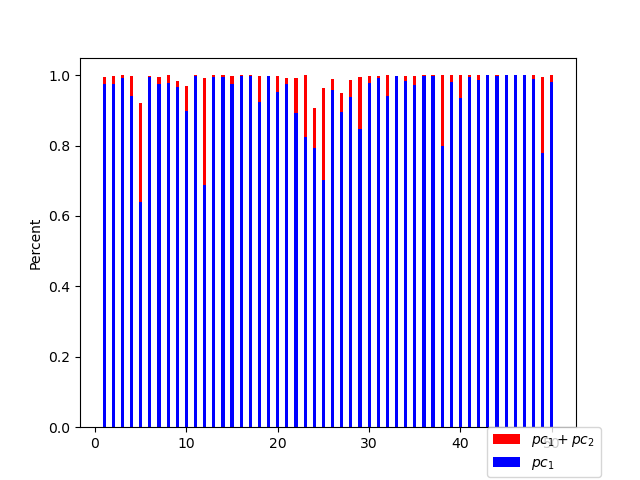
\includegraphics[width=0.7\textwidth,height=0.5\textwidth]{pca1.png}
	\caption{PCA result with 2 principal components by sklearn}
\end{figure}
\par 然后, 根据最大化方差的观点,若设$\mathbf{x}$是$m$维随机变量,$\Sigma$是$\mathbf{x}$的协方差矩阵,$\Sigma$的特征值从大到小依次是$\lambda_{1},\lambda_{2},\dots,\lambda_{m}\ge0$,其对应的特征向量依次是$\alpha_{1},\alpha_{2},\dots,\alpha_{m}$,则$\mathbf{x}$对应的第$k$主成分是$y_{k}=\alpha_{k}\dot x$,其主成分占比为$\frac{\lambda_{k}}{\sum_{i=1}^{m}\lambda_{i}}$.
\par 进而编写了函数$mypca(data,n=2,m=6,t=10)$.其中,$data=matrix$表示要做主成分的数据集,其中这个矩阵的行表示每个feature的不同观测,列表示不同的feature.$n$为保留的主成分数,$m$为随机变量的维数,事实上默认通过输入矩阵计算得出,$t$为时间窗的长度.通过该方法得到的结果如下:
\begin{figure}[H]
	\centering
	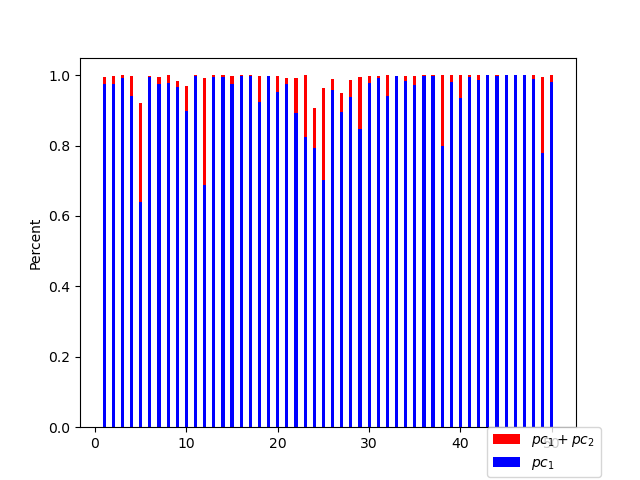
\includegraphics[width=0.7\textwidth,height=0.5\textwidth]{pca2.png}
	\caption{PCA result with 2 principal components by myself}
\end{figure}
\par 通过对比可以发现两种方法求得的PCA第一主成分和第二主成分的占比还是较为接近的.

\section{Ex2}
\par 首先考虑较为简单的Newton法.Newton法即每次前进的方向为$-H^{-1}\nabla\mathbf{f}$,其中$H$为目标函数的Hessian矩阵,$\nabla\mathbf{f}$为目标函数的梯度.Newton法有着较快的收敛速度,但是在实验中也出现了较多的问题:
\begin{figure}[htbp]
	\centering
	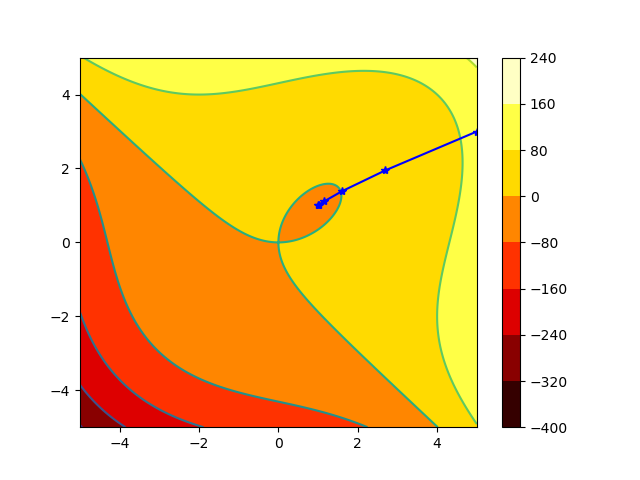
\includegraphics[width=0.7\textwidth,height=0.5\textwidth]{newton1.png}
	\caption{Newton method with initial $\mathbf{x}=(1,2)^{T}$}
\end{figure}
\par 可以发现经过短暂几步的迭代,Newton法就停止了搜索,探究其原因,是因为在$\mathbf{x}=(1,1)^{T}$处函数$\mathbf{f}$的梯度为0,此时Newton法不能再更新.
而$\mathbf{x}=(1,1)^{T}$点的Hessian矩阵为$\begin{pmatrix}
	6&-3\\
	-3&6
\end{pmatrix}$,其一阶子式为6,二阶子式为27,故为正定矩阵,此时$\mathbf{x}=(1,1)^{T}$为极小值点.这也可以看出Newton法极快的收敛速度.如图3:
\par 但是在某些初值,例如$\mathbf{x}=(-2,-1)^{T}$处,由于Newton法的学习率是固定的,会出现在迭代的不同时期,算法的步长出现过长或过小的情况,如图4:
\begin{figure}[htbp]
	\centering
	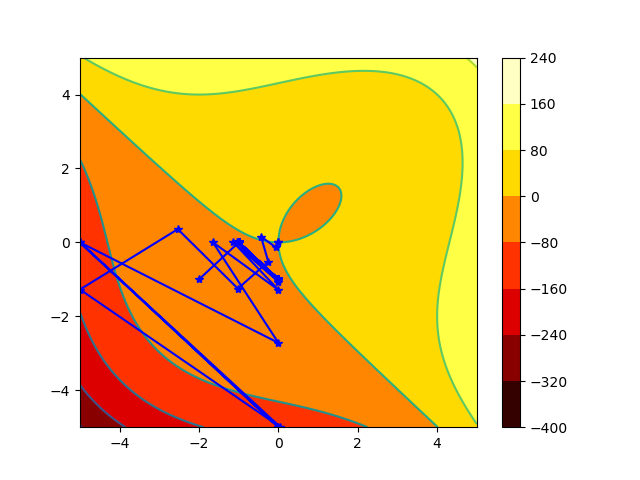
\includegraphics[width=0.7\textwidth,height=0.5\textwidth]{newton2.png}
	\caption{Newton method with initial $\mathbf{x}=(-2,-1)^{T}$}
\end{figure}
\par 事实上,引入自适应的步长能够解决这一问题,例如Adagrad以及著名的Adam算法.
\par \textbf{而对于最速下降法,由于每一步的搜索步长,或者说学习率,都相当于求解一个一维搜索问题,故是随着迭代的进行而不断变化的,因此可以找到正确的下降方向(这里我加了边界限制,否则的话会跑到$-\infty$...),对于某些初值(如$\mathbf{x}=(-0.01,-0.03)^{T}$),会趋向于"全局最小值"$(-\infty,-\infty)$,}如图5:
\begin{figure}[htbp]
	\centering
	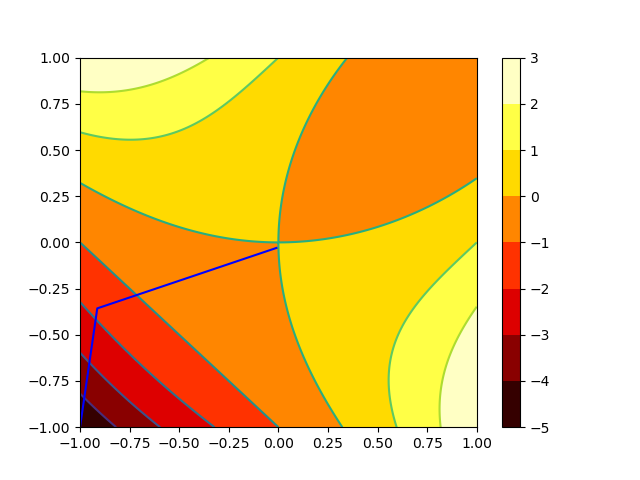
\includegraphics[width=0.7\textwidth,height=0.5\textwidth]{zuisu1.png}
	\caption{FastedDescent method with initial $\mathbf{x}=(-0.01,-0.03)^{T}$}
\end{figure}
\par 对于某些初值,例如$\mathbf{x}=(0.01,0.03)^T$,该算法会收敛到局部极小值点,如$\mathbf{x}=(1,1)^{T}$,如图6:
\begin{figure}[htbp]
	\centering
	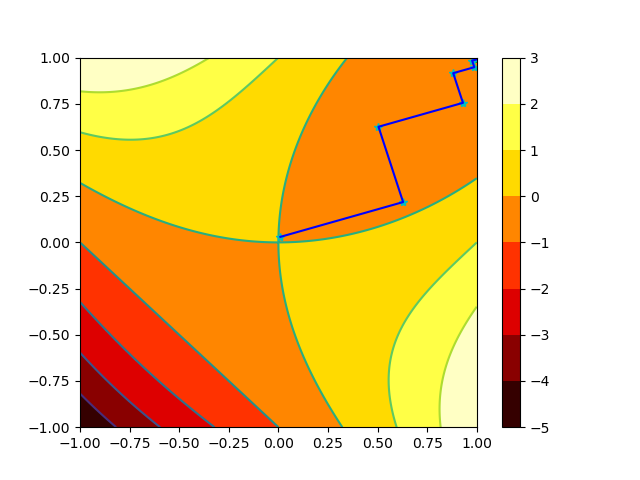
\includegraphics[width=0.7\textwidth,height=0.5\textwidth]{zuisu2.png}
	\caption{FastedDescent method with initial $\mathbf{x}=(0.01,0.03)^{T}$}
\end{figure}
\par \textbf{但是无论是对于Newton法还是最速下降法,一旦初值选为$(0,0)$,算法都不会进行;同时,若某一步到达$(0,0)$点,算法也不会继续进行,因为$(0,0)$是鞍点,要克服鞍点问题需要引入momentum(动量).}此外,由于在最速下降法中,每次迭代都要执行一次一维搜索(\textbf{尽管我采用了收敛较快的斐波那契法,同时通过先求解斐波那契表的方法提高了算法效率,但速度还是相对慢}),\textbf{算法的效率是较低的,梯度下降系列算法则可以很好的解决这一问题,其中考虑最为全面的亦是Adam算法,下将介绍并实现Adam算法(但是显然,本例中还不涉及样本的概念).}
\begin{algorithm}[H]
	\caption{Adam算法}  
	\begin{algorithmic} %每行显示行号  
		\Require 步长$\epsilon$.
		\Require 矩估计的指数衰减速率,$\rho_{1},\rho_{2}\in[0,1)$.
		\Require 用于数值稳定的较小常数$\delta$.
		\Require 初始参数$\mathbf{\theta}$.
		\Require 初始化一阶和二阶矩变量$s=0,r=0$.
		\Require 初始化时间步$t=0$. 
		\While{没有达到停止准侧}\\
		\qquad 从训练集中采集包含$m$个样本${x^{1},\dots,x^{m}}$的小批量,对应目标为$y^{i}$.\\
		\qquad 计算梯度:$\mathbf{g} \gets \frac{1}{m}\nabla_{\theta}\sum_{i}L(f(x^{i},\mathbf{\theta}),y^{i})$.\\
		\qquad $t\gets t+1$.\\
		\qquad 更新有偏一阶估计:$\mathbf{s}\gets \rho_{1}\mathbf{s}+(1-\rho_{1})\mathbf{g}$.\\
		\qquad 更新有偏二阶估计:$\mathbf{r}\gets \rho_{2}\mathbf{r}+(1-\rho_{2})\mathbf{g}\bigodot\mathbf{g}$.\\
		\qquad 修正一阶矩的偏差:$\hat{\mathbf{s}}\gets \frac{s}{1-\rho_{1}^{t}}$.\\
		\qquad 修正二阶矩的偏差:$\hat{\mathbf{r}}\gets \frac{r}{1-\rho_{2}^{t}}$.\\
		\qquad 计算更新:$\Delta \mathbf{\theta}=-\epsilon\frac{\hat{\mathbf{s}}}{\sqrt{\hat{\mathbf{r}}}+\delta}$.(逐元素应用操作)\\
		\qquad 应用更新:$\mathbf{\theta}\gets\mathbf{\theta}+\Delta\mathbf{\theta}$.
		\EndWhile  
		
	
	\end{algorithmic}  
\end{algorithm}  
\par 而在ADAM: A METHOD FOR STOCHASTIC OPTIMIZATION原文中的伪代码如图7:
\begin{figure}[htbp]
	\centering
	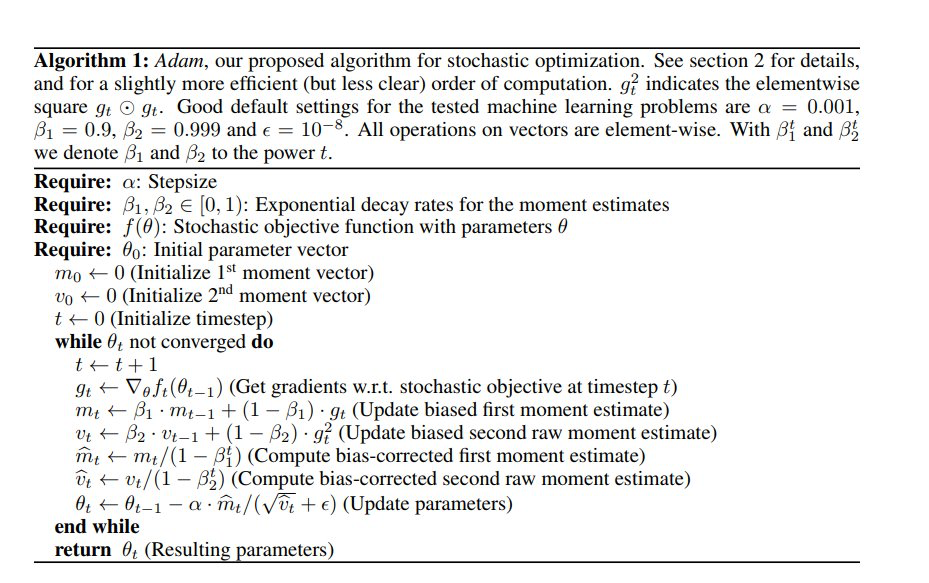
\includegraphics[width=0.9\textwidth,height=0.7\textwidth]{adam0.png}
	\caption{Pseudocode of Adam in original paper}
\end{figure}
\par 最后展示一下Adam的结果,它只用了17步就收敛到了接近$(1,1)$的位置:
\begin{figure}[H]
	\centering
	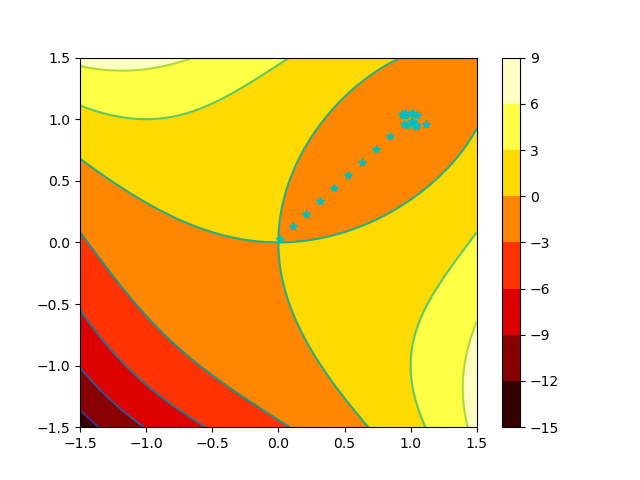
\includegraphics[width=0.7\textwidth,height=0.5\textwidth]{adam1.png}
	\caption{Adam method with initial $\mathbf{x}=(0.01,0.03)^{T}$}
\end{figure} 

\section{一点体会}
\par \textbf{初值选择真的很重要!初值选择真的很重要!初值选择真的很重要!}
\begin{thebibliography}{3}  
	\bibitem{ref1} 李航. 统计学习方法[M]. 清华大学出版社, 2012.
	\bibitem{ref2} Kingma D , Ba J . Adam: A Method for Stochastic Optimization[J]. Computer Science, 2014.
	\bibitem{ref3} Goodfellow, Ian, et al. Deep Learning[M]. MIT Press, 2016. 	
\end{thebibliography}
\end{document}
